\documentclass[conference,letterpaper]{IEEEtran}

% Packages sanctioned by IEEE
\usepackage{cite} % Compacts [1]--[4] citations and adds spaces
\usepackage[cmex10]{amsmath}
\usepackage[ruled, linesnumbered, noend]{algorithm2e}
\usepackage[caption=false,font=footnotesize]{subfig} % Good subfigures
\usepackage{array} % Better arrays
\usepackage{url}
\ifCLASSINFOpdf
  \usepackage[pdftex]{graphicx}
  \DeclareGraphicsExtensions{.pdf,.jpeg,.jpg,.png}
\else
  \usepackage[dvips]{graphicx}
  \DeclareGraphicsExtensions{.eps}
\fi
% Labels in IEEE format
% Equation
\newcommand{\eref}[1]{(\ref{#1})}
% Section
\newcommand{\sref}[1]{Section~\ref{#1}}
% Figure
\newcommand{\figref}[1]{Fig.\ref{#1}}
% Algorithm 
\newcommand{\algref}[1]{Algorithm~\ref{#1}}
% Algorithm 
\newcommand{\alglineref}[2]{line~\ref{#1}.\ref{#2}}


% Other useful packages
\usepackage{amssymb}
\usepackage{color}
\usepackage{booktabs}
\usepackage{verbatim}

% Insert hyperlinks in the document
\usepackage{hyperref}
\hypersetup{letterpaper,bookmarksopen,bookmarksnumbered,
pdfpagemode=UseOutlines,
colorlinks=true,
linkcolor=blue,
anchorcolor=blue,
citecolor=blue,
filecolor=blue,
menucolor=blue,
urlcolor=blue
}


%\algsetup{indent=2em}

\newtheorem{definition}{Definition}[section]
\newtheorem{property}{Property}[section]
\newtheorem{corollary}{Corollary}[section]
\newtheorem{propose}{Proposition}[section]
\newtheorem{theorem}{Theorem}[section]
\newtheorem{lemma}{Lemma}[section]
\newtheorem{example}{Example}[section]

\usepackage{ifthen,version}
\usepackage{color}
\newboolean{include-notes}
% Comment out the following line to exclude notes.
\setboolean{include-notes}{true}
%notes
\newcommand{\ssnote}[1]{\ifthenelse{\boolean{include-notes}}%
 {\textcolor{blue}{\textbf{SS: #1}}}{}}


\begin{document}
{\title{
Real-time Surface Reconstruction on a Mobile Device using Chunked Truncated
Signed Distance Fields }}
\author
{
	\IEEEauthorblockN
	{
		Matthew Klingensmith 
	}
	\IEEEauthorblockA
	{
		The Robotics Institute, Carnegie Mellon University\\
		\texttt{mklingen@andrew.cmu.edu}
	}
	\and
	\IEEEauthorblockN
	{
		Ivan Dryanovski
	}
	\IEEEauthorblockA
	{
		 City College of New York\\
		\texttt{ivan.dryanovski@gmail.com}
	}	
}

\maketitle

\begin{figure}[!t]
% Always try to place the figure on top of a column to save space
\centering
% Use linewidth to adjust width
% Use textheight(the total height of the column of text) to adjust height
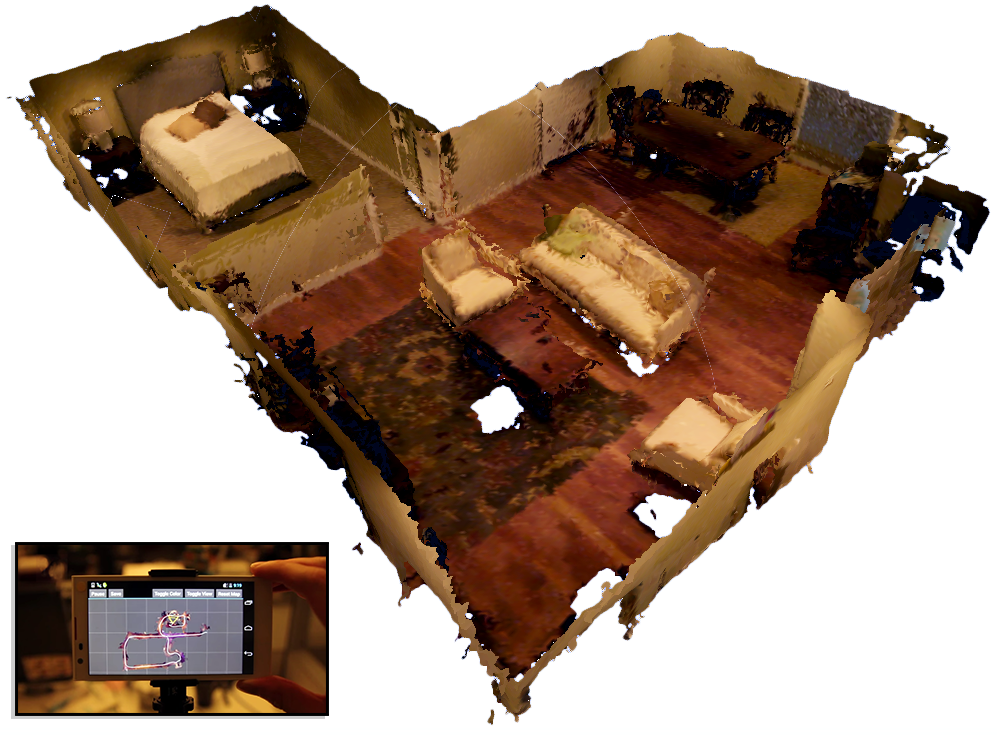
\includegraphics[width=\columnwidth]{img/fancycomposite}
\caption{An indoor apartment scene reconstructed in real-time on a mobile device
(inset) at a resolution of 3 cm.}
\label{fig:best}
\end{figure}

\textbf{Summary.}
In this work, we present an efficient algorithm for reconstructing 3D surfaces
on a depth sensor equipped mobile device in real-time using chunked, truncated
signed distance fields. 

\textbf{What is the problem?} 
We are interested in the problem of real-time 3D reconstruction. The task is to
extract the true 3D geometry and color of a real scene from a sequence of noisy
sensor readings from a handheld mobile device.

\textbf{Why is it interesting?} 
Solutions to this problem are useful for mobile robot navigation,
indoor localization, mapping, and object scanning.  As far as we know,
high-quality, real-time 3D surface reconstruction on a mobile device has never
been attempted before.

\textbf{Why is it hard?}
 The problem is ill-posed, since it requires localization as well as mapping
 (and hence is a variant of the SLAM problem.) In 3D, memory requirements for
 high quality 3D reconstruction are prohibitive. Real-time 3D reconstruction
 remains challenging on mobile devices.  Compared to full-sized machines, mobile
 devices have severely limited processing power, memory requirements, and
 graphics capabilities. Further, the depth sensors available on these devices
 are much more limited than their full-sized counterparts; they are typically
 lower resolution, have slower refresh rates, and have much more undesirable
 nonlinear distortion and noise.

\textbf{What is our insight?} 
Previous work on high quality real-time 3D reconstruction has focused on much
more capable and high-powered computing platforms with much more accurate
sensing, and is therefore not well suited for low-powered mobile devices. These
approaches, such as \textit{Kinect Fusion} \cite{Newcombe}, and
\textit{Kintinuous} \cite{Whelan2013}, work by costructing a truncated signed
distance field of the scene.

So far, real-time 3D reconstruction on mobile devices has been limited to simple
occupany grid mapping, using fixed 3D arrays \cite{Elfes1989, Newcombe}, and
octrees \cite{Wurm2010} which is not suitable for high quality 3D suface
 reconstruction.

Our main insight is to use a hybrid data structure containing a dynamic map of
fixed 3D ``chunks'' of signed distance field data.  Unlike fixed 3D arrays, this
data structure has much better memory performance; and, unlike octrees, it has
much better cache performance and boasts $\mathcal{O}(1)$ access times. By
chunking the distance field dynamically, we are able to asynchronously
reconstruct surfaces for rendering while new sensor data is coming in.

Additionally, by sacrificing the physical accuracy of raycasting for a more
efficient projection-based technique of constructing the distance field, we are
able to use \textit{negative information} in the form of space carving
\cite{Klingensmith2014} to produce a less noisy surface estimate.

\textbf{Contributions.} 
We make the following contributions:
\begin{itemize}
\item{An efficient data structure for representing very large volumetric data
sets.}
\item {An example framework and interface for doing large 3D reconstructions on
a mobile device.}
\item {Efficient techniques for real-time rendering and interaction with large
reconstructions on a mobile device.}
\end{itemize}

\textbf{Limitations.}
Our work depends on localization as a pre-requisite, and uses a visual intertial
odometry system as a black box input.  We make no attempt to improve
localization using mapping, and thus avoid the SLAM problem.  As such, our
reconstructions suffer from localization errors that we accumulate over time.
How can we use the map itself to improve pose estimates? We are interested in
using the volumetric signed distance data directly to compute global  
localization updates. 

\begin{figure*}[!t]
% Always try to place the figure on top of a column to save space
\centering
% Use linewidth to adjust width
% Use textheight(the total height of the column of text) to adjust height
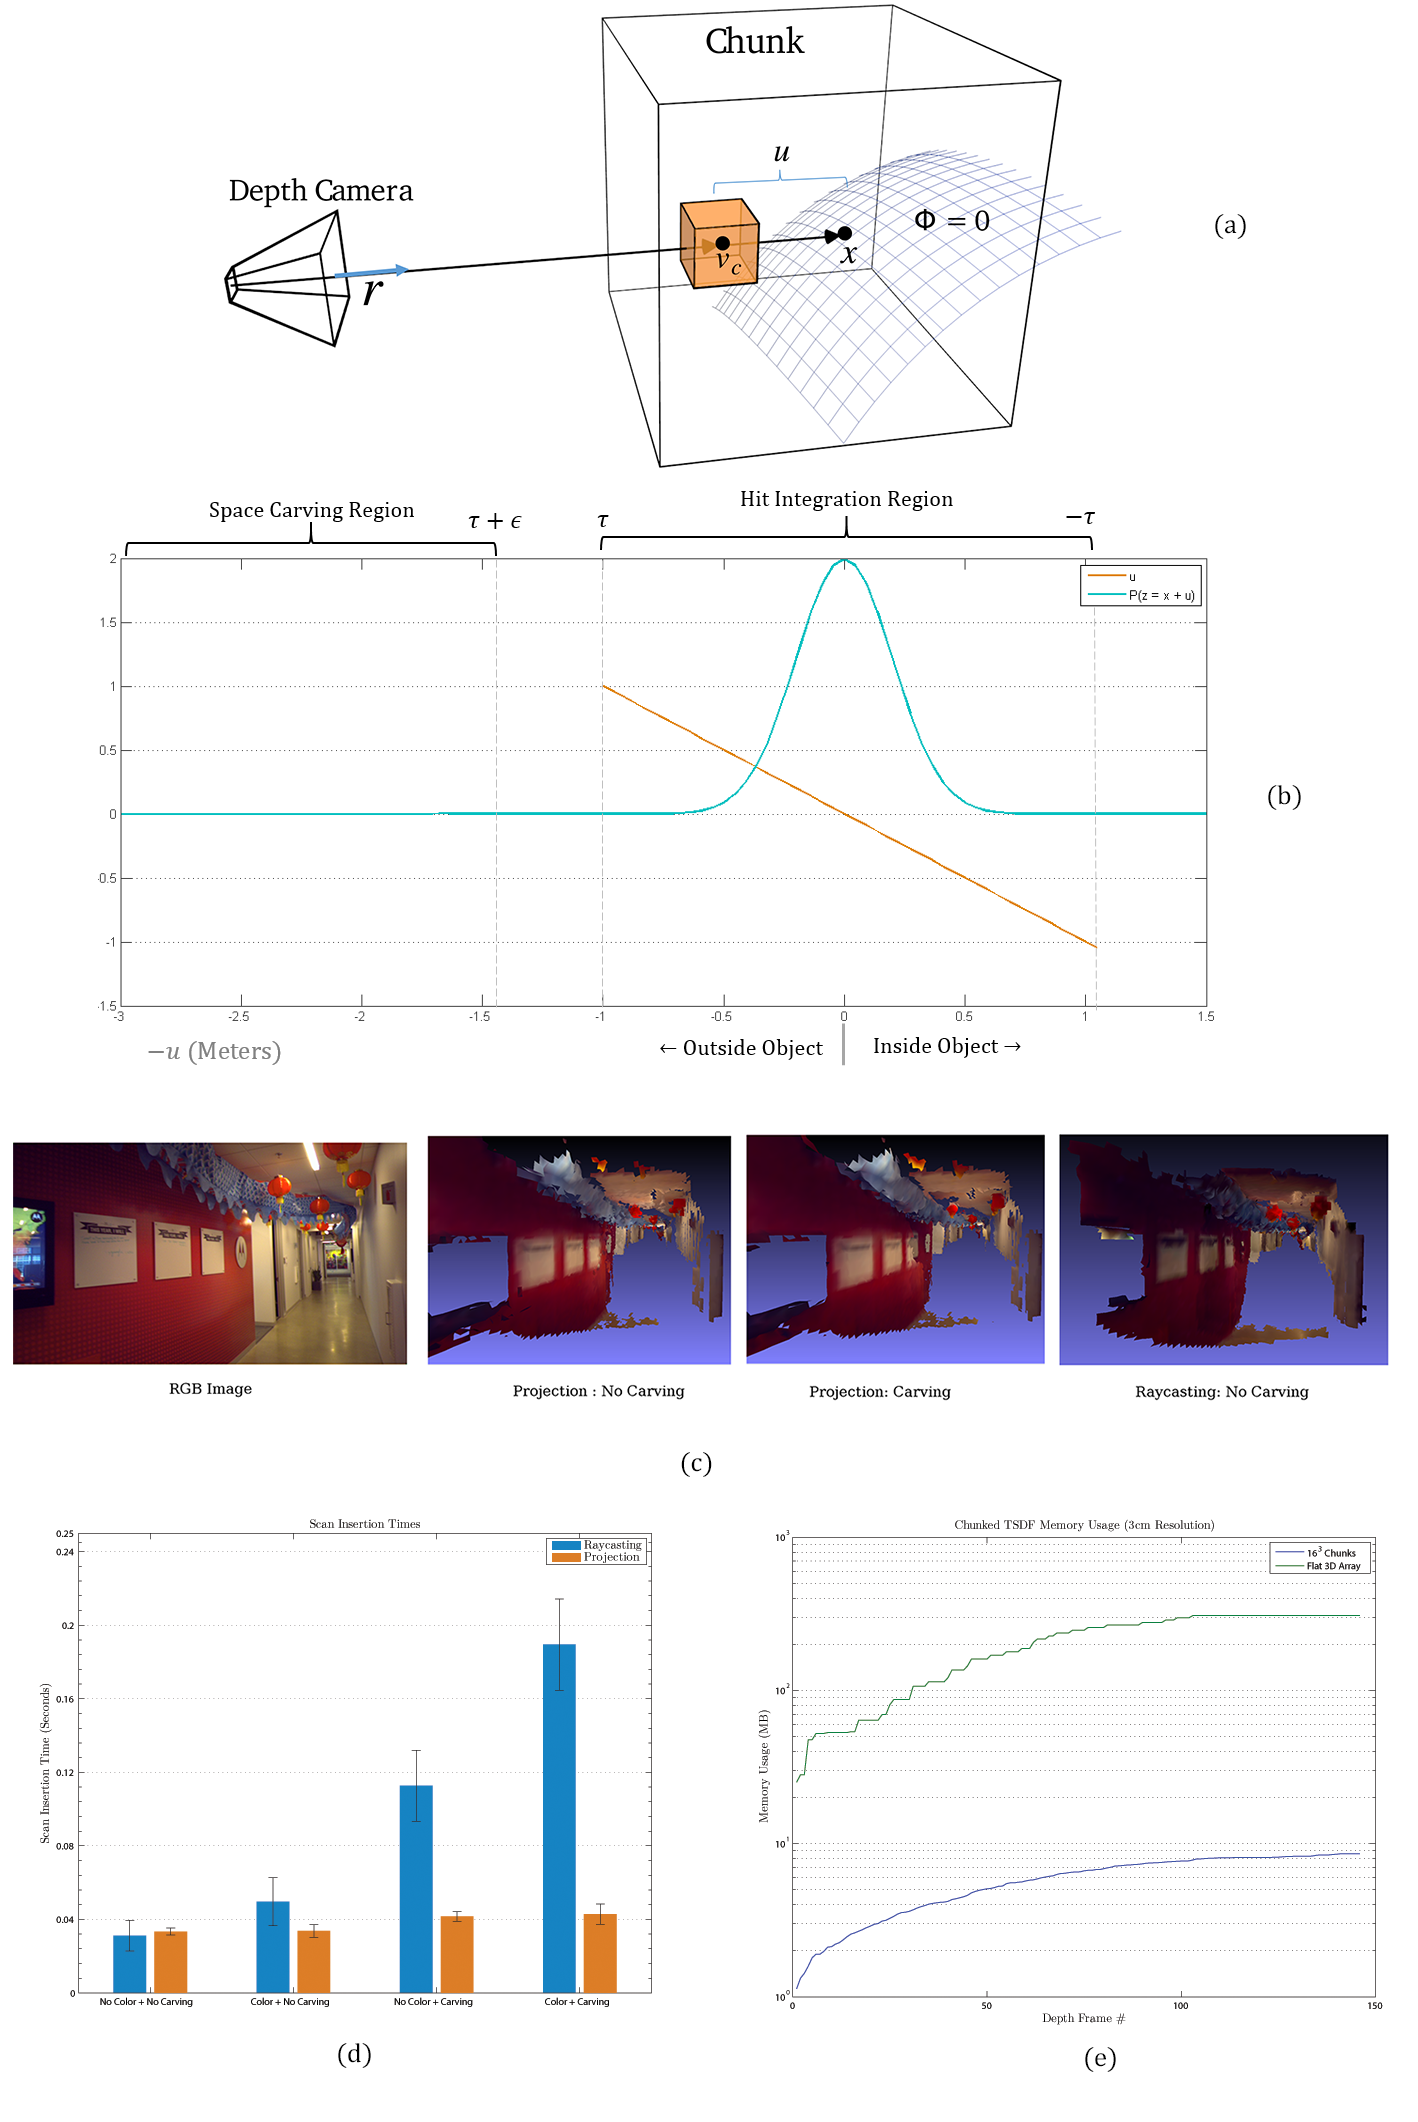
\includegraphics[width=0.62\linewidth]{img/bigpicture} 
%\framebox[\linewidth]{{\LARGE Explain the entire paper in one figure.}}
\caption{We divide the world into a series of chunks that contain $N_c^3$
voxels each. In each voxel we store the value of a signed distance function,
$\Phi(x)$. Wherever $Phi=0$, we have the surface. Wherever $\Phi < 0$, it is
inside an object, and vice versa wherever $\Phi > 0$. The distance field is
estimated near the surface by the distance along the depth ray from the surface
to the camera (a), within a threshold $\tau$ called the truncation distance
(b). In all parts of the space closer than $\tau + \epsilon$ to the camera, we
``carve'' voxels there. In all parts of the space within $\tau$ of the end of a
depth ray, we increment a running weighted average of voxels in the distance
field. Raycasting is approximated by a projection technique which has
resolution dependant accuracy (c), but which is much faster when space carving
is used (d). By only storing ``chunks'' of data near the surfaces of objects,
we use orders of magnitude less memory than \textit{Kinect Fusion} (e).}
\label{summary}
\end{figure*}

\bibliography{references}
\bibliographystyle{IEEEtran}
% Supplementary material
%\newpage
%\pagestyle{empty}
%\newpage
%\input{facilities.tex}


\end{document}